%\documentclass[wcp,gray]{jmlr} % test grayscale version
\documentclass[wcp]{jmlr}

% The following packages will be automatically loaded:
% amsmath, amssymb, natbib, graphicx, url, algorithm2e

%\usepackage{rotating}% for sideways figures and tables
\usepackage{longtable}% for long tables

% The booktabs package is used by this sample document
% (it provides \toprule, \midrule and \bottomrule).
% Remove the next line if you don't require it.
\usepackage{booktabs}
% The siunitx package is used by this sample document
% to align numbers in a column by their decimal point.
% Remove the next line if you don't require it.
%\usepackage[load-configurations=version-1]{siunitx} % newer version
%\usepackage{siunitx}

% The following command is just for this sample document:
\newcommand{\cs}[1]{\texttt{\char`\\#1}}

% This is required for dmath (display math)
\usepackage{breqn}

% To use multirow feature in table
\usepackage{multirow}

\jmlrvolume{29}
\jmlryear{2013}
\jmlrworkshop{ACML 2013}

\title[MML Laplace]{Minimum Message Length Estimate of Parameters of Laplace Distribution}

 % Use \Name{Author Name} to specify the name.
 % If the surname contains spaces, enclose the surname
 % in braces, e.g. \Name{John {Smith Jones}} similarly
 % if the name has a "von" part, e.g \Name{Jane {de Winter}}.
 % If the first letter in the forenames is a diacritic
 % enclose the diacritic in braces, e.g. \Name{{\'E}louise Smith}

 % Two authors with the same address
 % \author{\Name{Author Name1} \Email{abc@sample.com}\and
 %  \Name{Author Name2} \Email{xyz@sample.com}\\
 %  \addr Address}

 % Three or more authors with the same address:
 % \author{\Name{Author Name1} \Email{an1@sample.com}\\
 %  \Name{Author Name2} \Email{an2@sample.com}\\
 %  \Name{Author Name3} \Email{an3@sample.com}\\
 %  \Name{Author Name4} \Email{an4@sample.com}\\
 %  \Name{Author Name5} \Email{an5@sample.com}\\
 %  \Name{Author Name6} \Email{an6@sample.com}\\
 %  \Name{Author Name7} \Email{an7@sample.com}\\
 %  \Name{Author Name8} \Email{an8@sample.com}\\
 %  \Name{Author Name9} \Email{an9@sample.com}\\
 %  \Name{Author Name10} \Email{an10@sample.com}\\
 %  \Name{Author Name11} \Email{an11@sample.com}\\
 %  \Name{Author Name12} \Email{an12@sample.com}\\
 %  \Name{Author Name13} \Email{an13@sample.com}\\
 %  \Name{Author Name14} \Email{an14@sample.com}\\
 %  \addr Address}


 % Authors with different addresses:
  \author{\Name{Parthan Kasarapu} \Email{parthan.kasarapu@monash.edu}\\
  \addr Faculty of IT, Monash University, Clayton, VIC 3800, Australia
  \AND
  \Name{Lloyd Allison} \Email{lloyd.allison@monash.edu}\\
  \addr Faculty of IT, Monash University, Clayton, VIC 3800, Australia
  \AND
  \Name{Enes Makalic} \Email{emakalic@unimelb.edu.au}\\
  \addr Centre for MEGA Epidemiology, The University of Melbourne, Carlton, VIC 3053, Australia
 }

\editor{Cheng Soon Ong and Tu Bao Ho}
% \editors{List of editors' names}

\begin{document}

\maketitle

\begin{abstract}
The Laplace distribution offers a number of uses in statistical inference and
modelling on symmetric data with long tails. We report here for the first time
the derivation of the minimum message length (MML) estimates of location ($\mu$) and 
scale ($b$) parameters of the Laplace distribution for any observed data. 
We demonstrate an application of this work to compare and contrast the
quality of orthogonal superposition of two (spatial) vector sets under 
$L^1$ and $L^2$ norm.
\end{abstract}

\begin{keywords}
Laplace distribution, Normal distribution, MML, Monte Carlo simulation
\end{keywords}

\section{Introduction}
Laplace distribution is a continuous probability density function which is dependent on
the absolute value of the difference between the mean and the data point. Because of
this characteristic, inference of parameters of this distribution (based on some 
empirical data) is not severely affected in the presence of outliers. Laplace distribution
is a model of choice in areas as diverse as signal processing 
\citep{laplace-signal-processing}, image denoising \citep{image-denoising},
gene expression studies \citep{Bhowmick01102006}, market risk prediction
\citep{haas2005modeling}, and machine learning \citep{Cord:2006:FSR:1167556.1167570}.
In most of these applications, a mixture model of Laplace distributions is used. 

Normal distribution, on the other hand, is sensitive to outliers because of the quadratic 
nature of the contributions of individual terms. In the presence 
of outliers, the inference of parameters is skewed to dampen the effect of their residuals 
with respect to the model. In many problems, formulating an objective function (that needs 
to be optimized) as sum of squared deviations (the $L^2$ norm) results in a closed
form solution. Its $L^1$ equivalent, however, does not have an analytical solution
(for data with more than one dimension). 

We show this in the context of superposition of vector sets and use Monte Carlo simulation
to optimize the objective function when it is formulated using $L^1$ norm. We compare
the superpositions resulting from using the two versions of objective functions
using the minimum message length (MML) criterion. MML is used to adjudicate which is 
better on individual test cases. 

The MML expression for the Normal distribution has been 
worked out previously \citep{wallace68,WallaceBook}, while the MML estimates for the Laplace 
distribution have not been characterized. 
The main contribution of this work is the derivation of the message length 
expression and estimation of the MML parameters for the Laplace distribution.
The general procedure to formulate the message length expression for transmitting
data using some statistical model is outlined in \citet{wallace-87} and is 
referred to as Strict Message Length (SMML) Inference. This is computationally
infeasible and is shown to be NP-hard \citep{Farr01012002}. \citet{wallace-87}
provide an approximate form which is commonly referred to as the 
\emph{Wallace-Freeman} approximation. The MML method
of estimating parameters for a number of distributions using this approximation
has been well established \citep{WallaceBook}. In this paper, we use the 
Wallace-Freeman's quadratic approximation
to derive the the message length expression for the Laplace distribution. 

MML is an information theoretic way of Bayesian inference \citep{wallace68}. MML is best
understood through a communication process between an imaginary pair of transmitter
and receiver connected over a Shannon channel. The method involves
encoding the model and its fit to the data. A model that results in the smallest total message
length is inferred as the most suitable under this criterion. Indeed the message length
paradigm provides an objective means to differentiate between competing models
and select the best one. In this paper, we use this intuition to 
evaluate the overall fit when the data is modelled  using a Normal and a Laplace distribution. 

The results demonstrate the use of Laplace estimates in two cases. 
The first scenario involves data being randomly
generated from a Laplace distribution. This data is then fitted using
both Normal and Laplace models. We use the derived formulation of Laplace MML to
compute the Laplace fit. This is then compared against the fit using a Normal
distribution. 

As a demonstration of a practical real world application, we consider the problem of
superposition of vector sets. The objective function for the superposition problem can be formulated
where the deviations of the corresponding vectors are calculated using the $L^1$ norm 
or the $L^2$ norm. In MML parlance, the optimal superposition would correspond to stating
the deviations concisely. We encode the deviations using both Normal and Laplace
distributions. The distribution which results in the best compression is chosen
to be the best model for those two vector sets.

\section{The Minimum Message Length (MML) Framework}
\subsection{Inductive Inference}
\citet{wallace68} developed the first practical criterion for model selection using 
information theory. MML provides an elegant framework to compare any two competing 
hypotheses that model some observed data. The hypothesis that results in the shortest 
overall message length is chosen as the best one, in line with traditional statistical 
inference using the Bayesian method.\footnote{http://allisons.org/ll/MML/} Using 
Bayes's theorem to explain some observed data $D$ by hypothesis $H$, we get:
$$\Pr(H\&D) = \Pr(H) \times \Pr(D|H) = \Pr(D) \times \Pr(H|D)$$
where $\Pr(H\&D)$ is the joint probability of data $D$ and hypothesis $H$, $\Pr(H)$
is the prior probability of hypothesis $H$, $\Pr(D)$ is the prior probability of 
probability of data $D$, $\Pr(H|D)$ is the posterior probability of $H$
given $D$, and $\Pr(D|H)$ is the likelihood.
MML uses the following result from information theory: given an event $E$
with a probability $\Pr(E)$, the message length $I(E)$ for an optimal
code is given by $I(E) = -\log_2 (\Pr(E))$ bits \citep{shannon1948}. Applying this insight
to the Bayes's theorem, we get the following relationship between
conditional probabilities in terms of optimal message lengths:\[I(H\&D) = I(H) + I(D|H) = I(D) + I(H|D)\]
In the traditional Bayesian framework, the hypothesis $H$ with
the largest posterior probability $\Pr(H|D)$ is often preferred.
Among the terms in the above equation, $\Pr(H)$ (and hence $I(H)$) can
usually be estimated well for some \emph{reasonable} prior(s) on hypotheses.
Given the data $D$ and a chosen prior $H$, the likelihood $\Pr(D|H)$ can also be estimated.
Whilst comparing two competing hypotheses, the prior of observed data $\Pr(D)$
can be ignored as it is a common factor. Hence, for two competing hypotheses, $H$ and $H^\prime$, we have:
$$I(H|D) - I(H^\prime|D) = I(H) + I(D|H) - I(H^\prime) - I(D|H^\prime)$$
The discriminative ability of MML lies in its consideration of the model
complexity and the error of the fit. In the MML setting, the net message,
therefore, involves statement cost of the hypothesis
(given by $I(H)$) and statement cost of the data given the hypothesis (given by $I(D|H)$). 

\subsection{Parameter Estimation using MML}
The hypothesis is a statistical model which is characterized by its parameters.
MML accounts for both the model complexity and its explanatory power of the 
data observed. MML works by maximizing the expectation of the posterior
probability and this is where it differs from the traditional Bayesian methods.
This involves determining the \emph{accuracy of parameter values (AOPV)} for
continuous parameters. AOPV is a measure of the uncertainty in stating a
parameter and it is this region over which the expectation is maximized. As per
MML, a parameter need not be stated very accurately. The optimal precision to which
it needs to be stated is computed as part of the MML inference. A good
description of the procedure is outlined in \citet{oliver1994mml}. 

\section{Message Length of Laplace distribution}
\citet{wallace-87} derived the approximation to the code length of the two part message as
\begin{align}
I(\bar{\theta},D) &= I(\bar{\theta}) + I(D|\bar{\theta}) \notag\\
&\approx \underbrace{\frac{d}{2}\log\kappa_d -\log h(\bar{\theta}) + \frac{1}{2}\log(det\,F(\bar{\theta}))}_{\mathrm{part 1}} + \underbrace{L(\bar{\theta}) + \frac{d}{2}}_{\mathrm{part 2}} \label{eqn:wf_msglen}
\end{align}
where $\bar{\theta}$ is the set of model parameters, $d$ is the number of parameters, 
$\kappa_d$ is the $d$-dimensional lattice quantization constant \citep{conwaySloane84}, 
$h(\bar{\theta})$ is the prior probability of the parameters, 
$det(\mathrm{F}(\bar{\theta}))$ is the determinant of the expected Fisher matrix, and
$L(\bar{\theta})$ is the negative log likelihood of observed data. The MML estimates 
$\hat{\bar{\theta}}_{\mathrm{MML}}$ of the parameters are determined by minimizing 
\eqref{eqn:wf_msglen}. 

\subsection{Laplace distribution}
The contribution of this paper is in the derivation of the MML estimates of 
the parameters of the Laplace distribution which have not been characterized previously.
The parameters describing a Laplace distribution are the location($\mu$) and the scale ($b$).
The probability density function (pdf) is given in \eqref{eqn:laplace_pdf}.
\begin{equation}
\mathrm{pdf}(x) = \frac{1}{2b}\mathrm{exp}\left(-\frac{|x-\mu|}{b}\right) \label{eqn:laplace_pdf}
\end{equation}
To derive the MML estimates, we use the Wallace-Freeman approximation \citep{wallace-87}. 
This estimation as per \eqref{eqn:wf_msglen} requires the likelihood function, the Fisher information matrix,
and the  prior distributions on the parameters. Let $D = \{x_1,x_2,\ldots,x_N\}$ be the observed data 
containing $N$ samples and $\epsilon$ be the precision to which each datum is stated. 
Let $\mathrm{R}_{\mu}$, $\mathrm{R}_{b}$ be the range of $\mu$ and $\log b$ 
respectively ($\epsilon$, $\mathrm{R}_{\mu}$, $\mathrm{R}_{b}$ are hyperparameters
which are introduced in \citet{WallaceBook}). Using \eqref{eqn:laplace_pdf},
the \emph{likelihood function} is given by
\[ f(D|\bar{\theta}) = \prod_{n=1}^N \frac{\epsilon}{2b} e^{-\frac{|x_n-\mu|}{b}} \]
and, hence, the \emph{negative log-likelihood} is computed as
\begin{align}
 L(\bar{\theta}) &= -\log f(D|\bar{\theta}) \notag\\
		 &= N\log\left(\frac{2}{\epsilon}\right) + N\log b + \frac{1}{b}\sum_{n=1}^N |x_n-\mu| \label{eqn:laplace_l}
\end{align}
The maximum likelihood (ML) estimates for $\mu$ and $b$ are given by
\begin{align*}
\hat{\mu}_{\mathrm{ML}} &= \mathrm{median}\{x_n\} \\ 
\hat{b}_{\mathrm{ML}} &= \frac{1}{N} \sum_{n=1}^N |x_n-\hat{\mu}_{\mathrm{ML}}|
\end{align*}

\subsection*{Computation of Fisher information $\mathbf{F(\bar{\boldsymbol{\theta}})}$}
The Fisher information matrix is given by
\begin{align*}
  \mathrm{F}(\mu,b) &= \left( \begin{array}{cc}
  \mathrm{E} \left[\frac{\partial^2 L}{\partial \mu^2}\right] & \mathrm{E} \left[\frac{\partial^2 L}{\partial\mu \partial b}\right] \\
  \mathrm{E} \left[\frac{\partial^2 L}{\partial b \partial\mu}\right] & \mathrm{E} \left[\frac{\partial^2 L}{\partial b^2}\right] 
  \end{array} \right) 
\end{align*}
where $\mathrm{E}[.]$ is the expected value of that quantity. Using \eqref{eqn:laplace_l},
\begin{align*}
 \frac{\partial^2 L}{\partial b^2} &= -\frac{N}{b^2} + \frac{2}{b^3} \sum_{n=1}^N |x_n-\mu| \\
 \mathrm{E} \left[\frac{\partial^2 L}{\partial b^2}\right] &= -\frac{N}{b^2} + \frac{2}{b^3} \mathrm{E}\left[\sum_{n=1}^N |x_n-\mu|\right]
\end{align*}
\begin{align*}
 \mathrm{E}\left[|x-\mu|\right] &= \int\limits_{-\infty}^{\infty} |x-\mu| . \frac{1}{2b} . e^{-\frac{|x-\mu|}{b}} dx \\
 &= \frac{1}{2b} \int\limits_{-\infty}^{\mu} -(x-\mu) e^{\frac{(x-\mu)}{b}} dx + \int\limits_{\mu}^{\infty} (x-\mu)e^{-\frac{(x-\mu)}{b}} dx \\
 &= b
\end{align*}
\begin{equation}
 \mathrm{Therefore,}\quad \mathrm{E} \left[\frac{\partial^2 L}{\partial b^2}\right] = -\frac{N}{b^2} + \frac{2}{b^3} (Nb) = \frac{N}{b^2} \label{eqn:fisher_44} 
\end{equation}
%The computation of $\mathrm{E}\left[\frac{\partial^2 L}{\partial \mu^2}\right]$ and 
%$\mathrm{E}\left[\frac{\partial^2 L}{\partial \mu \partial b}\right]$ is involved and hence,
%tucked away in \autoref{apd:laplace_fisher}. Using those results, we have
%\section{Derivations involved in the computation of Laplace Fisher}
%\label{apd:laplace_fisher}
\begin{align*}
 \frac{\partial L}{\partial \mu} &= -\frac{1}{b} \sum_{n=1}^N \frac{(x_n-\mu)}{|x_n-\mu|} \quad\quad\left(\mathrm{using} \frac{d}{dx}|x| = \frac{d}{dx}\sqrt{x^2} = \frac{x}{|x|}\right)
\end{align*}
This is discontinuous as it is piecewise constant. Hence to calculate $\frac{\partial^2 L}{\partial \mu^2}$, the following approach is adopted: 
Assume that the actual distribution has parameters $m$ and 
$b$. The receiver, however, decodes the mean as $\mu$ to an accuracy of parameter
value $\delta$. As such $\mu$ is a random variable and it is fair to reason out
that $\mu \in \left[m-\frac{\delta}{2},m+\frac{\delta}{2}\right]$. It is 
assumed that $\mu$ follows a uniform distribution in this range. Using this 
assumption, now we compute the $\mathrm{E}\left[\frac{\partial L}{\partial \mu}\right]$ 
and subsequent calculations. From our assumptions, $\mathrm{pdf}(\mu) = \frac{1}{\delta}$.
\begin{align*}
 \therefore \frac{\partial L}{\partial \mu} &\approx \mathrm{E}\left[\frac{\partial L}{\partial \mu}\right] = -\frac{1}{b}\mathrm{E}\left[\sum_{n=1}^{N}\frac{x_n-\mu}{|x_n-\mu|}\right]
\end{align*}
\begin{align*}
 \mathrm{E}\left[\frac{x-\mu}{|x-\mu|}\right] &= \int\limits_{-\infty}^{\infty} \frac{x-\mu}{|x-\mu|}.\frac{1}{2b}.e^{\frac{|x-m|}{b}} dx \\
 &= \int\limits_{-\infty}^{\mu} -\frac{1}{2b} e^{-\frac{|x-m|}{b}} dx + \int\limits_{\mu}^{\infty} \frac{1}{2b} e^{-\frac{|x-m|}{b}} dx
\end{align*}
(i) Let $\mu < m$
\begin{align*}
 \therefore \mathrm{E}\left[\frac{x-\mu}{|x-\mu|}\right] &= \int\limits_{-\infty}^{\mu} -\frac{1}{2b} e^{\frac{x-m}{b}} dx + \int\limits_{\mu}^{m} \frac{1}{2b} e^{\frac{x-m}{b}} dx + \int\limits_{m}^{\infty} \frac{1}{2b} e^{-\frac{x-m}{b}} dx \\
 &= 1 - e^{\frac{\mu-m}{b}}
\end{align*}
(ii) Let $\mu > m$
\begin{align*}
 \therefore \mathrm{E}\left[\frac{x-\mu}{|x-\mu|}\right] &= \int\limits_{-\infty}^{m} -\frac{1}{2b} e^{\frac{x-m}{b}} dx + \int\limits_{m}^{\mu} -\frac{1}{2b} e^{-\frac{x-m}{b}} dx + \int\limits_{\mu}^{\infty} \frac{1}{2b} e^{-\frac{x-m}{b}} dx \\
 &= -(1 - e^{-\frac{\mu-m}{b}})
\end{align*}
(i) and (ii) can be merged and hence, $\mathrm{E}\left[\frac{x-\mu}{|x-\mu|}\right] = - sgn(\mu-m) (1 - e^{-\frac{|\mu-m|}{b}})$. From the argument above,
\begin{align}
 \frac{\partial L}{\partial \mu} &\approx \mathrm{E}\left[\frac{\partial L}{\partial \mu}\right] = -\frac{1}{b} \mathrm{E}\left[\sum_{n=1}^{N}\frac{x_n-\mu}{|x_n-\mu|}\right]\notag\\
 &= \frac{N}{b} sgn(\mu-m) (1 - e^{-\frac{|\mu-m|}{b}}) \label{eqn:laplace_expected_approx}\\
 \therefore \frac{\partial^2 L}{\partial \mu^2} &= \frac{N}{b^2} e^{\frac{-|\mu-m|}{b}} \notag\\
 \mathrm{E} \left[\frac{\partial^2 L}{\partial \mu^2}\right] &= \frac{N}{b^2} \mathrm{E}\left[e^{\frac{-|\mu-m|}{b}}\right] \notag
\end{align}
\begin{align*}
 \mathrm{E}\left[e^{\frac{-|\mu-m|}{b}}\right] &= \int\limits_{m-\frac{\delta}{2}}^{m+\frac{\delta}{2}} e^{\frac{-|\mu-m|}{b}} . \frac{1}{\delta} . d\mu \\
 &= \frac{1}{\delta} \int\limits_{m-\frac{\delta}{2}}^{m} e^{\frac{\mu-m}{b}} d\mu + \int\limits_{m}^{m+\frac{\delta}{2}}e^{-\frac{\mu-m}{b}} d\mu \\
 &= 2b \left(\frac{1-e^{-\frac{\delta}{2b}}}{\delta}\right) \\
 &= 2b \left( \frac{1}{2b} - \frac{1}{2b}\mathcal{O}\left(\frac{\delta}{2b}\right) \right) \quad\quad(\mathrm{assuming} \quad \delta \ll 2b) \\
 &\approx 1
 \end{align*}
\begin{equation}
 \mathrm{Therefore,}\quad \mathrm{E} \left[\frac{\partial^2 L}{\partial \mu^2}\right] = \frac{N}{b^2} (1) = \frac{N}{b^2} \label{eqn:fisher_11}
\end{equation}
Using \eqref{eqn:laplace_expected_approx}, 
\begin{align*}
 \frac{\partial^2 L}{\partial b \partial \mu} &= N sgn(\mu-m) \left[ -\frac{1}{b^2} - \left( e^{\frac{-|\mu-m|}{b}} \left( -\frac{1}{b^2} \right) + \frac{1}{b} e^{\frac{-|\mu-m|}{b}} \frac{|\mu-m|}{b^2} \right) \right] \\
 &= -\frac{N}{b^2} sgn(\mu-m)(1-e^{-\frac{|\mu-m|}{b}}) - \frac{N}{b} . \frac{(\mu-m)}{b^2} . e^{-\frac{|\mu-m|}{b}} \\
 \mathrm{Therefore,}\quad \mathrm{E} \left[\frac{\partial^2 L}{\partial b \partial \mu}\right] &= -\frac{N}{b^2} (\mathrm{E}_1 - \mathrm{E}_2) - \frac{N}{b^3} \mathrm{E}_3, \quad\quad\mathrm{where}
\end{align*}
\begin{align*}
 \mathrm{E}_1 &= \mathrm{E}[sgn(\mu-m)] = \int\limits_{m-\frac{\delta}{2}}^{m+\frac{\delta}{2}} sgn(\mu-m).\frac{1}{\delta}.d\mu = \frac{1}{\delta} \int\limits_{m-\frac{\delta}{2}}^{m+\frac{\delta}{2}} \frac{\mu-m}{|\mu-m|} d\mu \\
 &= \frac{1}{\delta} \int\limits_{-\frac{\delta}{2}}^{\frac{\delta}{2}} \frac{t}{|t|} dt = 0 \quad\quad(\mathrm{as\,\,the\,\,integrand\,\,is\,\,an\,\,odd\,\,function})
\end{align*}
\begin{align*}
 \mathrm{E}_2 &= \mathrm{E}[sgn(\mu-m)e^{-\frac{|\mu-m|}{b}}] = \frac{1}{\delta} \int\limits_{m-\frac{\delta}{2}}^{m+\frac{\delta}{2}} \frac{\mu-m}{|\mu-m|} e^{-\frac{|\mu-m|}{b}} d\mu \\
 &= \frac{b}{\delta} \int\limits_{-\frac{\delta}{2}}^{\frac{\delta}{2}} \frac{t}{|t|} e^{-|t|} dt = 0 \quad\quad(\mathrm{as\,\,the\,\,integrand\,\,is\,\,an\,\,odd\,\,function})
\end{align*}
\begin{align*}
 \mathrm{E}_3 &= \mathrm{E}[(\mu-m)e^{-\frac{|\mu-m|}{b}}] = \frac{1}{\delta} \int\limits_{m-\frac{\delta}{2}}^{m+\frac{\delta}{2}} (\mu-m)e^{-\frac{|\mu-m|}{b}} d\mu \\
 &= \frac{b^2}{\delta} \int\limits_{-\frac{\delta}{2}}^{\frac{\delta}{2}} t e^{-|t|} dt = 0 \quad\quad(\mathrm{as\,\,the\,\,integrand\,\,is\,\,an\,\,odd\,\,function})
\end{align*}
\begin{equation} 
  \mathrm{Therefore,}\quad \mathrm{E} \left[\frac{\partial^2 L}{\partial b \partial \mu}\right] = 0 \label{eqn:fisher_22} 
\end{equation}
Using \eqref{eqn:fisher_44}, \eqref{eqn:fisher_11}, \eqref{eqn:fisher_22},
\begin{align*}
  \mathrm{F}(\mu,b) &= \left( \begin{array}{cc}
        \frac{N}{b^2} & 0 \\
        0 & \frac{N}{b^2}
            \end{array} \right) 
\end{align*}
\begin{equation} \mathrm{Therefore,}\quad det(\mathrm{F}(\mu,b)) = \frac{N^2}{b^4} \label{eqn:laplace_fisher} \end{equation}

\subsection*{Priors on the parameters}
A prior probability on $\mu$ and $b$ is assumed in accordance with the prior assumed
in the case of Normal. The ranges from which $\mu$ and $\log b$ are drawn are prespecified as 
$\mathrm{R}_{\mu}$ and $\mathrm{R}_{b}$ respectively \citep{WallaceBook}. 
\begin{align} 
\therefore h(\bar{\theta}) = h(\mu,b) &= h(\mu) h(b) \notag\\
      &= \frac{1}{\mathrm{R}_{\mu}}. \frac{1}{b \mathrm{R}_{b}} \label{eqn:laplace_h} 
\end{align}

Using \eqref{eqn:wf_msglen}, \eqref{eqn:laplace_fisher}, \eqref{eqn:laplace_h},
\begin{dmath*}
 I(\mu,b) = \left( \log\kappa_2 + \log(\mathrm{R}_{\mu}\mathrm{R}_{\sigma}) + \log N - \log b \right) + \left( N\log\left(\frac{2}{\epsilon}\right) + N\log b + \frac{1}{b}\sum_{n=1}^N |x_n-\mu| + 1 \right)
\end{dmath*} 

\noindent To obtain the MML estimates $\hat{\mu}_{\mathrm{MML}}$ and $\hat{b}_{\mathrm{MML}}$ 
which results in minimum $I$, $\frac{\partial I}{\partial \mu} = 0$ and 
$\frac{\partial I}{\partial b} = 0$. The MML estimates are therefore, given by
\begin{align}
  \hat{\mu}_{\mathrm{MML}} &= \mathrm{median}\{x_n\} \notag\\
  \hat{b}_{\mathrm{MML}} &= \frac{1}{N-1} \sum_{n=1}^N |x_n-\hat{\mu}_{\mathrm{MML}}| 
  \label{eqn:laplace_estimate}
\end{align}
The corresponding minimized message length is given as
\begin{dmath}
 \therefore I_{min} = I(\hat{\mu}_{\mathrm{MML}},\hat{b}_{\mathrm{MML}}) = 1 + \log\kappa_2 + \log(\mathrm{R}_{\mu}\mathrm{R}_{\sigma}) + \log N + N\log\left(\frac{2}{\epsilon}\right) + (N-1) \log \left( \frac{\sum_{n=1}^N |x_n-\hat{\mu}_{\mathrm{MML}}|}{N-1} \right) + (N-1) \label{eqn:laplace_mml_estimate}
\end{dmath} 

\section{MML Inference for a Normal distribution}
A Normal distribution whose density function (pdf) is given by \eqref{eqn:normal_pdf}
\begin{equation}
\mathrm{pdf}(x) = \frac{1}{\sqrt{2\pi}\sigma} \mathrm{exp}\left(-\frac{(x-\mu)^2}{2\sigma^2}\right) \label{eqn:normal_pdf}
\end{equation}
is characterized by the mean $\mu$ and the standard deviation $\sigma$. The MML estimates 
for a Normal distribution is presented in \citet{WallaceBook,wallace-87} and are:
\begin{align*}
\hat{\mu}_{\mathrm{MML}} &= \frac{1}{N} \sum_{n=1}^N x_n \\
\hat{\sigma}_{\mathrm{MML}}^2 &= \frac{\sum_{n=1}^N (x_n-\hat{\mu}_{\mathrm{MML}})^2}{N-1}
\end{align*}
The corresponding minimized message length is given as
\begin{dmath}
 \therefore I_{min} = I(\hat{\mu}_{\mathrm{MML}},\hat{\sigma}_{\mathrm{MML}}) = 1 + \log\kappa_2 + \log(\mathrm{R}_{\mu}\mathrm{R}_{\sigma}) + \frac{1}{2}\log(2N^2) + \frac{N}{2}\log\left(\frac{2\pi}{\epsilon^2}\right) + \frac{N-1}{2}\log\left(\frac{\sum_{n=1}^N (x_n-\hat{\mu}_{\mathrm{MML}})^2}{N-1}\right) + \frac{N-1}{2}  \label{eqn:normal_mml_estimate}
\end{dmath} 
As established in \citet{wallace-87}, the optimal precision to which the parameters need
to be stated is given by: $AOPV \propto \frac{1}{\sqrt{det(F(\bar{\theta}))}}$.
The Normal Fisher is $\frac{2N^2}{\sigma^4}$ \citep{WallaceBook} and the Laplace Fisher 
as derived above is $\frac{N^2}{b^4}$. There is a marked difference in the optimal AOPVs
computed in the two cases. For the same value of spread ($\sigma=b$), the uncertainty in
the parameter values for a Laplace is $\sqrt{2}$ times that of Normal, which means
that the parameters for a Laplace need to be stated less precisely when compared with the Normal.

\section{Experiments}
We demonstrate the use of Laplace estimates in two scenarios. 

\subsection{Data generation and modelling}
In the first case, data is generated randomly from a distribution (Normal \& Laplace) 
separately. This data is then modelled using the two distributions.
It is observed that if the true distribution is a Laplace/Normal, then the
compression in message length is better when it is modelled using a Laplace/Normal
distribution. This is indeed expected and is done as a validation check to ensure that 
the derived MML formulation for the Laplace is consistent with the observation.
\eqref{eqn:laplace_mml_estimate} and \eqref{eqn:normal_mml_estimate} are used to determine
the code length when the data is modelled using the Laplace and Normal distributions
respectively. 

As an example, 500 random samples are generated from each of the distributions.
The mean of the true distribution is taken to be 0 and the spread (standard
deviation $\sigma$ for a Normal and scale parameter $b$ for a Laplace) is
chosen to be 2. \autoref{fig:data_approximation} shows the original distributions
and the corresponding Normal and Laplace approximations. In \autoref{fig:normal_data},
the true distribution is normal (red curve). The Normal approximation (blue curve)
overlaps almost entirely with the red curve which is an indication of a good fit.
The Laplace approximation (green curve) significantly deviates from the original
distribution. The same argument holds for \autoref{fig:laplace_data} where the
underlying distribution of the data is Laplace, and hence, in this case, the Laplace
seems to be a good fit. 

\autoref{tab:comparison_estimates} provides a comparison of the estimates of the
two distributions. The message length (msglen) is computed in bits. It can be seen
when the true distribution is Laplace, the message length corresponding to the Laplace 
estimate (6690.91 bits) is smaller compared to that of the Normal estimate (6755.68 bits).

\begin{figure}[!htb]
  \centering
    \subfigure[Original distribution: Normal]
    {
      \centering
        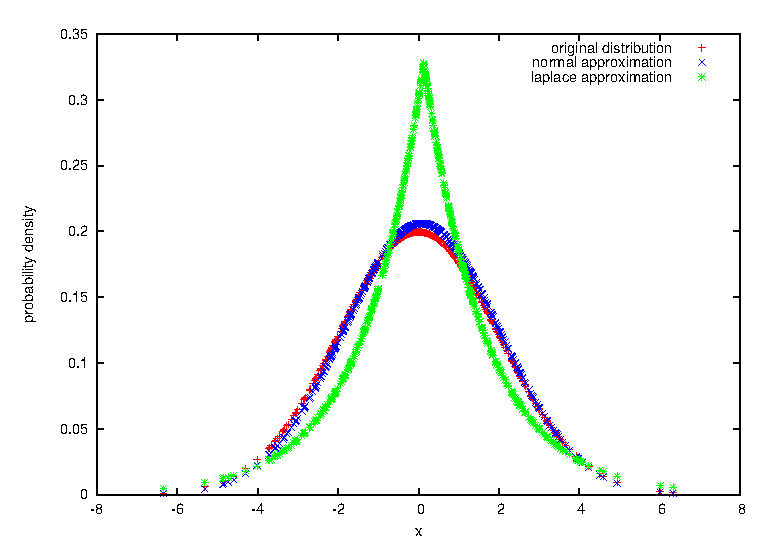
\includegraphics[width=0.45\textwidth]{fig/normal_n_500_mean_0_scale_2.eps}
        \label{fig:normal_data}
    }
    \hspace{0.5cm}
    \subfigure[Original distribution: Laplace]
    {
        \centering
        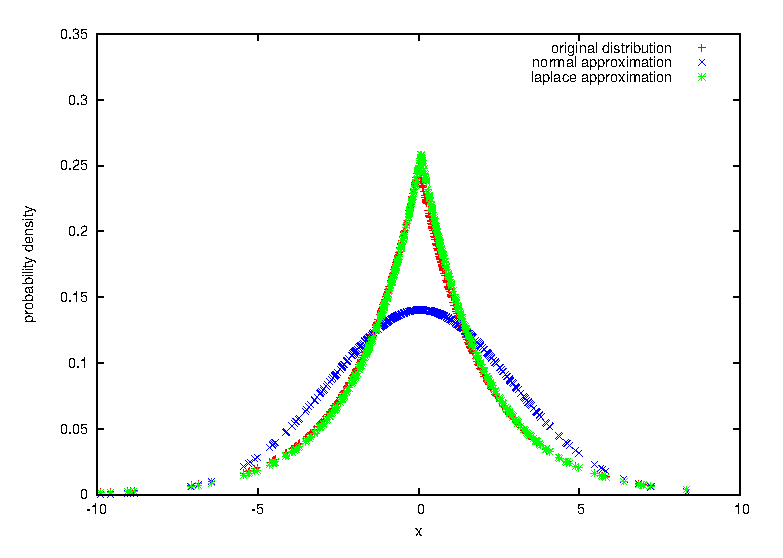
\includegraphics[width=0.45\textwidth]{fig/laplace_n_500_mean_0_scale_2.eps}
        \label{fig:laplace_data}
    }
    \caption{Approximation of data using Normal \& Laplace distributions}
    \label{fig:data_approximation}
\end{figure}

\begin{table}[h]
\centering
\caption{Comparison of the estimates}
\label{tab:comparison_estimates}
\begin{tabular}{|c|c|c|c|c|c|c|c|c|}
\hline
True & True & True & \multicolumn{3}{c|}{Normal estimates} & \multicolumn{3}{c|}{Laplace estimates} \\ \cline{4-9} 
distribution & mean & spread & mean & spread & msglen & mean & spread & msglen \\ \hline 
Normal & 0 & 2 & 0.0722611 & 1.93638 & 6493.89 & 0.127191 & 1.52389 & 6518 \\ \hline
Laplace & 0 & 2 & -0.0455104 & 2.78563 & 6755.68 & 0.0471194 & 1.9376 & 6690.91 \\ \hline
\end{tabular}
\end{table}

\begin{figure}[!htb]
  \centering
    \subfigure[Original distribution: Normal]
    {
      \centering
        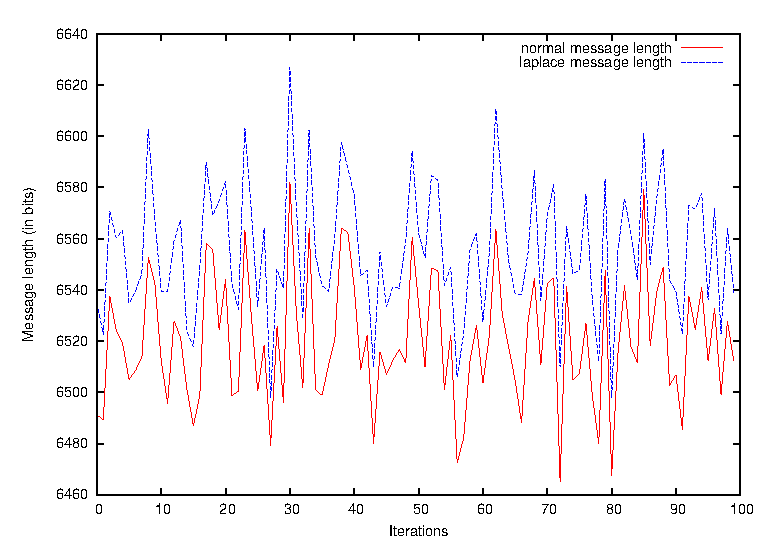
\includegraphics[width=0.45\textwidth]{fig/statistics_normal_n_500_mean_0_scale_2.eps}
        \label{fig:normal_data_iterations}
    }
    \hspace{0.5cm}
    \subfigure[Original distribution: Laplace]
    {
        \centering
        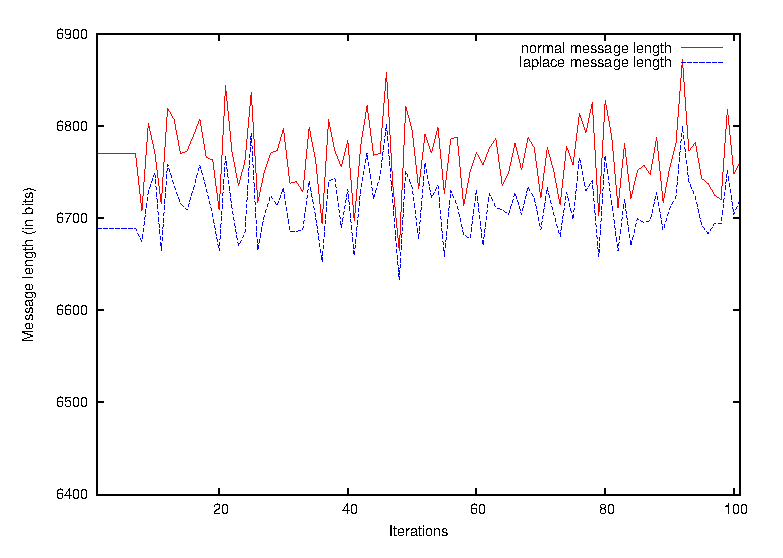
\includegraphics[width=0.45\textwidth]{fig/statistics_laplace_n_500_mean_0_scale_2.eps}
        \label{fig:laplace_data_iterations}
    }
    \caption{Comparison of message lengths over many iterations}
    \label{fig:data_approximation_iterations}
\end{figure}

\autoref{fig:data_approximation_iterations} compares the message lengths over 100 iterations.
In \autoref{fig:normal_data_iterations}, the original distribution is Normal and it is observed
that over all the iterations, the message length for the Normal (red) is consistently less than that
of the Laplace (blue). In \autoref{fig:laplace_data_iterations}, the original distribution is 
Laplace and it is observed that over all the iterations, the message length for the Laplace (blue) 
is consistently less than that of the Normal (red).

\subsection{Superposition of vector sets}
Given any two vector sets $U = \{u_1,u_2,\ldots,u_m\}$ and $V = \{v_1,v_2,\ldots,v_m\}$
where each $u_i$ and $v_i$, $(i \in \{1,2,\ldots,m\})$ is a vector in 3D space, the 
superpositioning problem refers to finding a suitable transformation on $U$ to
align it with $V$ such that the deviations of each vector in $V$ with its counterpart
in $U$ is minimum. Let the transformation be effected by a translation vector $t$ and a rotation matrix $R$.
Let it result in an altered vector set $U'=\{u_1',u_2',\ldots,u_m'\}$, where $u_i'=R(u_i-t)$.
The objective function corresponding to the sum of squares ($L^2$ norm) of all deviations: 
\begin{equation} 
  \sum_{i=1}^m \|v_i-u_i'\|^2 = \sum_{i=1}^m \|v_i-R(u_i-t)\|^2 \label{eqn:L2_objective_function}
\end{equation} 
and the objective function corresponding to the sum of absolute deviations ($L^1$ norm)
\begin{equation} 
  \sum_{i=1}^m \|v_i-u_i'\| = \sum_{i=1}^m \|v_i-R(u_i-t)\| \label{eqn:L1_objective_function}
\end{equation}
(where $\|.\|$ denotes the vector norm) needs to be minimized. 
The superposition problem can be formulated in the MML framework as finding the 
orientation of two proteins such that the deviations of each corresponding point
are encoded in an effective manner. Superposition based on minimizing total least
squares corresponds to stating the deviations using a Normal distribution. 
Superposition based on minimizing the absolute value of the deviations correspond
to transmitting the deviations using a Laplace distribution. \citet{keynes-laplace} 
showed that the Laplace distribution minimized the absolute deviation from the median
(which is also corroborated by the MML estimate of Laplace parameters 
\eqref{eqn:laplace_estimate}) and is, hence, pertinent for our current discussion. 

Minimization of \eqref{eqn:L2_objective_function} yields $t = \left(\frac{\sum_{i=1}^m u_i}{m} - \frac{R\sum_{i=1}^m v_i}{m}\right)$.
Substituting this value of $t$ in \eqref{eqn:L2_objective_function} results in the modified objective function:
\begin{equation}
\sum_{i=1}^m \left|\left|\left(v_i - \frac{\sum_{i=1}^m v_i}{m}\right) - R \left(u_i - \frac{\sum_{i=1}^m u_i}{m}\right)\right|\right|^2 \label{eqn:L2_after_translation}
\end{equation} 

\citet{kearsley89} provides a solution to \eqref{eqn:L2_objective_function} by 
resolving the transformation into translation and rotation. The centres of mass of the
two vector sets are translated to the origin \eqref{eqn:L2_after_translation} and the problem then reduces to finding the
rotation matrix which minimizes the total least squares. This involves respresenting
the rotation matrix using a quaternion and then solving the resultant eigen value 
decomposition problem. As such, \citet{kearsley89} offers an analytical way to solve
the \emph{least squares} superposition problem. 
 
Minimizing \eqref{eqn:L1_objective_function}, however, does not yield a closed form solution. 
Differentiating \eqref{eqn:L1_objective_function} with respect to $t$ and setting it to $0$ yields
\begin{equation}
\sum_{i=1}^m \frac{Rv_i-(u_i-t)}{\|Rv_i-(u_i-t)\|} = 0 \label{eqn:L1_after_translation}
\end{equation} 
In this case, $R$ and $t$ cannot be separated and hence, cannot be analytically solved for.
As such, one needs to adopt approximate methods to find the best superposition corresponding
to the $L^1$ norm. The one used in this paper is a version that uses Monte Carlo simulation. 
It is described below:
\begin{enumerate}
\item Apply Kearsley's transformation and find the superposition that corresponds
to least sum of squares of the deviations. In this state, the value of the 
objective function \eqref{eqn:L1_objective_function} is computed. 
\item From this orientation, the protein is perturbed randomly. If the new orientation
results in a better value of the L1 norm \eqref{eqn:L1_objective_function}, the new orientation is
accepted. If however, the value of the objective function is less than the previous
value, the new orientation is accepted with a minute probability.
\item This is repeated for many iterations. The process is expected to converge to
the global minimum. As such, this would correspond to the optimal
superposition which minimizes the sum of absolute deviations.
\end{enumerate}

The two vector sets are first superposed using the Kearsley's method and the message
length ($I_{N}$) computed through MML inference using a Normal distribution. 
Monte Carlo simulation is performed (as discussed above) from this stage and
the final orientation is obtained. At this point, the message length ($I_L$) is
computed through MML inference using a Laplace distribution. Two cases arise:-
\begin{itemize}
\item If $I_L < I_N$, then there exists a superposition which is optimal than the
one resulting from minimizing the sum of squared deviations \eqref{eqn:L2_objective_function}.
\item If $I_N < I_L$, then the superposition obtained by minimizing
\eqref{eqn:L2_objective_function} is better. Since the minimal L1 superposition
is obtained using a Monte Carlo simulation (which is terminated after a certain number
of iterations), it could also be possible that the optimal solution wasn't found.
\end{itemize}

The point of this exercise is to show that not all vector sets have their
optimal superpositions dictated by minimizing sum of squared deviations. It also drives
home the use of MML estimators in determining the kind of superposition to be
considered. 

\subsection*{Results}
We apply the problem of superposition to protein structures. The vector sets would
correspond to the three dimensional coordinates of the $\alpha$-carbon atoms of 
amino acid residues constituting the proteins' backbone. We use SUPER \citep{super}
(which is an implementation of Kearsley's orthogonal superposition)
to get all protein segments from the Protein Data Bank which fit to a Root Mean 
Squared Deviation (RMSD) of 5 Angstroms (\AA). The protein segment corresponding
to PDB ID 2IC7, chain A and residues 132-162 was randomly
considered and there were $\sim$23000 segments which fit within a RMSD of 5 \AA. 
The message length corresponding to this optimal $L^2$ superposition is calculated
using \eqref{eqn:normal_mml_estimate}. This orientation will also have a certain
value for the sum of absolute deviations. The message length to encode these
absolute differences is computed using \eqref{eqn:laplace_mml_estimate}.
For these 23000 segments across several proteins, we determine the optimal $L^1$ superposition
using Monte Carlo simulation. The superposition resulting after 1000 iterations
is regarded as the optimal $L^1$ superposition. The message length to encode the
absolute differences is computed. There were about $\sim$1700 instances where the
optimal $L^1$ superposition is better than the $L^2$ equivalent. A few 
results are discussed in \autoref{tab:comparison_mml}. 

The `moving structure' is the protein that is perturbed from its optimal $L^2$
superposition. Each segment is uniquely identified by its chain ID and residue span.
These are obtained using SUPER.
RMSD is the error of fit (in \AA) of the $L^2$ superposition. The initial/final
$L^1$ deviations correspond to the average of the absolute deviations (in \AA) 
in both these orientations;
msglen($L^2$) is the message length using a Normal distribution to encode the
deviations in the optimal $L^2$ superposition; msglen (initial $L^1$) corresponds to the
message length of encoding the absolute deviations before perturbations and msglen (final $L^1$)
is the message length to encode the deviations after the Monte Carlo simulation.
\begin{table}[h]
\centering
\caption{Comparison of the minimum message lengths}
\label{tab:comparison_mml}
\begin{tabular}{|c|c|c|c|c|c|c|}
\hline
Moving & \multirow{2}{*} {RMSD} & initial $L^1$ & Final $L^1$ & msglen & msglen & msglen \\
structure & & deviation & deviation & ($L^2$) & (initial $L^1$) & (final $L^1$) \\
\hline
3IG7 [A:139-169] & 1.834 & 1.910 & 1.814 & 1134.82 & 1102.03 & 1096.32 \\
4G87 [A:291-321] & 2.112 & 2.555 & 2.455 & 1153.54 & 1165.38 & 1145.22 \\
3R8Y [A:105-135] & 0.479 & 0.673 & 0.666 & 956.711 & 1063.82 & 1059.25 \\
\hline
\end{tabular}
\end{table}
As expected, the final $L^1$ deviation is less than the initial one. It is observed this happens for 
most of the cases which suggest the presence of the $L^1$ optimal value somewhere close
to the initial position. 

For the discussion below, in \autoref{fig:compare_structure_1}, \autoref{fig:compare_structure_2},
\autoref{fig:compare_structure_3}, the red curve corresponds to the fixed protein; the blue curve
is the optimal $L^2$ superposition, and the green curve corresponds to the optimal $L^1$ superposition.

The first row in \autoref{tab:comparison_mml} corresponds to \autoref{fig:compare_structure_1}.
Its msglen(initial $L^1$) < msglen($L^2$). This suggests that $L^1$ superposition supercedes 
the $L^2$ superposition, and it only gets better
as the structure is perturbed as is evidenced by the msglen(final $L^1$), the message length
after the Monte Carlo simulation. Here, it can be seen that the red curve (the fixed protein) 
is closer to the green curve ($L^1$ superposition) than to the blue curve ($L^2$ superposition)
in the majority of the protein structure.
\begin{figure}[!htb]
\centering
\includegraphics[scale=0.5]{fig/compare_structure_1.eps}
\label{fig:compare_structure_1}
\caption{Initial \& final $L^1$ superposition better than $L^2$ superposition}
\end{figure}
\begin{figure}[!htb]
  \centering
    \subfigure[Final $L^1$ superposition better than $L^2$ superposition]
    {
      \centering
        \includegraphics[width=0.45\textwidth]{fig/compare_structure_2.eps}
        \label{fig:compare_structure_2}
    }
    \hspace{0.5cm}
    \subfigure[$L^2$ superposition better than $L^1$ superposition]
    {
        \centering
        \includegraphics[width=0.45\textwidth]{fig/compare_structure_3.eps}
        \label{fig:compare_structure_3}
    }
    \caption{Comparing the protein superpositions with respect to $L^1$ and $L^2$ norm}
    \label{fig:protein_superposition}
\end{figure}
The second row in \autoref{tab:comparison_mml} corresponds to the case where the final $L^1$
superposition (1145.22 bits) is optimal than the $L^2$ superposition (1153.54 bits). The initial
$L^1$ superposition (1165.38 bits) is not the optimal one and hence, has to go through a series of
iterations to reach the local optimum. In \autoref{fig:compare_structure_2}, the green curve 
(final $L^1$) is better than $L^2$ superposition.
%\begin{figure}[!htb]
%\centering
%\includegraphics[scale=0.5]{fig/compare_structure_2.eps}
%\label{fig:compare_structure_2}
%\caption{Final $L^1$ superposition better than $L^2$ superposition}
%\end{figure}
The third row in \autoref{tab:comparison_mml} demonstrates the case where the $L^2$ superposition
(956.711 bits) is optimal compared to the $L^1$ superposition (1059.25 bits). On careful 
inspection, one can see the red curve (in \autoref{fig:compare_structure_3}) is closer
to the blue curve corresponding to the $L^2$ superposition than to the green curve ($L^1$ superposition).
%\begin{figure}[!htb]
%\centering
%\includegraphics[scale=0.5]{fig/compare_structure_3.eps}
%\label{fig:compare_structure_3}
%\caption{$L^2$ superposition better than $L^1$ superposition}
%\end{figure}

\section{Conclusion}
We have derived the MML estimators for the Laplace distribution and applied it
in the context of encoding the superposition of vector sets. This is used to
distinguish the quality of superposition for any two vector sets. 
In general, if the objective function is formulated as the sum of absolute differences,
we have a framework using MML to encode these values using 
a Laplace distribution. The quality of the overall fit can be evaluated using the
MML inference technique and can be compared with other models.
For the specific problem of superposition of two vector sets, the choice of $L^1$ or $L^2$
superposition is made by comparing the message lengths obtained by encoding deviations
using $L^1$ and $L^2$ norm.

\acks{TODO}

\bibliography{references}

\appendix
%\section{Derivations involved in the computation of Laplace Fisher}
%\label{apd:laplace_fisher}
%\begin{align*}
% \frac{\partial L}{\partial \mu} &= -\frac{1}{b} \sum_{n=1}^N \frac{(x_n-\mu)}{|x_n-\mu|} \quad\quad\left(\mathrm{using} \frac{d}{dx}|x| = \frac{d}{dx}\sqrt{x^2} = \frac{x}{|x|}\right)
%\end{align*}
%This is discontinuous as it is piecewise constant. Hence to calculate $\frac{\partial^2 L}{\partial \mu^2}$, the following approach is adopted: \\\\
%Assume that the actual distribution has parameters $m$ and 
%$b$. The receiver, however, decodes the mean as $\mu$ to an accuracy of parameter
%value $\delta$. As such $\mu$ is a random variable and it is fair to reason out
%that $\mu \in \left[m-\frac{\delta}{2},m+\frac{\delta}{2}\right]$. I_1t is 
%assumed that $\mu$ follows a uniform distribution in this range. Using this 
%assumption, now we compute the $\mathrm{E}\left[\frac{\partial L}{\partial \mu}\right]$ 
%and subsequent calculations. From our assumptions, $\mathrm{pdf}(\mu) = \frac{1}{\delta}$.
%\begin{align*}
% \therefore \frac{\partial L}{\partial \mu} &\approx \mathrm{E}\left[\frac{\partial L}{\partial \mu}\right] = -\frac{1}{b}\mathrm{E}\left[\sum_{n=1}^{N}\frac{x_n-\mu}{|x_n-\mu|}\right]
%\end{align*}
%\begin{align*}
% \mathrm{E}\left[\frac{x-\mu}{|x-\mu|}\right] &= \int\limits_{-\infty}^{\infty} \frac{x-\mu}{|x-\mu|}.\frac{1}{2b}.e^{\frac{|x-m|}{b}} dx \\
% &= \int\limits_{-\infty}^{\mu} -\frac{1}{2b} e^{-\frac{|x-m|}{b}} dx + \int\limits_{\mu}^{\infty} \frac{1}{2b} e^{-\frac{|x-m|}{b}} dx
%\end{align*}
%(i) Let $\mu < m$
%\begin{align*}
% \therefore \mathrm{E}\left[\frac{x-\mu}{|x-\mu|}\right] &= \int\limits_{-\infty}^{\mu} -\frac{1}{2b} e^{\frac{x-m}{b}} dx + \int\limits_{\mu}^{m} \frac{1}{2b} e^{\frac{x-m}{b}} dx + \int\limits_{m}^{\infty} \frac{1}{2b} e^{-\frac{x-m}{b}} dx \\
% &= 1 - e^{\frac{\mu-m}{b}}
%\end{align*}
%(ii) Let $\mu > m$
%\begin{align*}
% \therefore \mathrm{E}\left[\frac{x-\mu}{|x-\mu|}\right] &= \int\limits_{-\infty}^{m} -\frac{1}{2b} e^{\frac{x-m}{b}} dx + \int\limits_{m}^{\mu} -\frac{1}{2b} e^{-\frac{x-m}{b}} dx + \int\limits_{\mu}^{\infty} \frac{1}{2b} e^{-\frac{x-m}{b}} dx \\
% &= -(1 - e^{-\frac{\mu-m}{b}})
%\end{align*}
%(i) and (ii) can be merged and hence, $\mathrm{E}\left[\frac{x-\mu}{|x-\mu|}\right] = - sgn(\mu-m) (1 - e^{-\frac{|\mu-m|}{b}})$. From the argument above,
%\begin{align}
% \frac{\partial L}{\partial \mu} &\approx \mathrm{E}\left[\frac{\partial L}{\partial \mu}\right] = -\frac{1}{b} \mathrm{E}\left[\sum_{n=1}^{N}\frac{x_n-\mu}{|x_n-\mu|}\right]\notag\\
% &= \frac{N}{b} sgn(\mu-m) (1 - e^{-\frac{|\mu-m|}{b}}) \label{eqn:laplace_expected_approx}\\
% \therefore \frac{\partial^2 L}{\partial \mu^2} &= \frac{N}{b^2} e^{\frac{-|\mu-m|}{b}} \notag\\
% \mathrm{E} \left[\frac{\partial^2 L}{\partial \mu^2}\right] &= \frac{N}{b^2} \mathrm{E}\left[e^{\frac{-|\mu-m|}{b}}\right] \notag
%\end{align}
%\begin{align*}
% \mathrm{E}\left[e^{\frac{-|\mu-m|}{b}}\right] &= \int\limits_{m-\frac{\delta}{2}}^{m+\frac{\delta}{2}} e^{\frac{-|\mu-m|}{b}} . \frac{1}{\delta} . d\mu \\
% &= \frac{1}{\delta} \int\limits_{m-\frac{\delta}{2}}^{m} e^{\frac{\mu-m}{b}} d\mu + \int\limits_{m}^{m+\frac{\delta}{2}}e^{-\frac{\mu-m}{b}} d\mu \\
% &= 2b \left(\frac{1-e^{-\frac{\delta}{2b}}}{\delta}\right) \\
% &= 2b \left( \frac{1}{2b} - \frac{1}{2b}\mathcal{O}\left(\frac{\delta}{2b}\right) \right) \quad\quad(\mathrm{assuming} \quad \delta \ll 2b) \\
% &\approx 1
% \end{align*}
%\begin{equation*}
% \therefore \mathrm{E} \left[\frac{\partial^2 L}{\partial \mu^2}\right] = \frac{N}{b^2} (1) = \frac{N}{b^2}
%\end{equation*}
%Using \eqref{eqn:laplace_expected_approx}, 
%\begin{align*}
% \frac{\partial^2 L}{\partial b \partial \mu} &= N sgn(\mu-m) \left[ -\frac{1}{b^2} - \left( e^{\frac{-|\mu-m|}{b}} \left( -\frac{1}{b^2} \right) + \frac{1}{b} e^{\frac{-|\mu-m|}{b}} \frac{|\mu-m|}{b^2} \right) \right] \\
% &= -\frac{N}{b^2} sgn(\mu-m)(1-e^{-\frac{|\mu-m|}{b}}) - \frac{N}{b} . \frac{(\mu-m)}{b^2} . e^{-\frac{|\mu-m|}{b}} \\
% \therefore \mathrm{E} \left[\frac{\partial^2 L}{\partial b \partial \mu}\right] &= -\frac{N}{b^2} (\mathrm{E}_1 - \mathrm{E}_2) - \frac{N}{b^3} \mathrm{E}_3, \quad\quad\mathrm{where}
%\end{align*}
%\begin{align*}
% \mathrm{E}_1 &= \mathrm{E}[sgn(\mu-m)] = \int\limits_{m-\frac{\delta}{2}}^{m+\frac{\delta}{2}} sgn(\mu-m).\frac{1}{\delta}.d\mu = \frac{1}{\delta} \int\limits_{m-\frac{\delta}{2}}^{m+\frac{\delta}{2}} \frac{\mu-m}{|\mu-m|} d\mu \\
% &= \frac{1}{\delta} \int\limits_{-\frac{\delta}{2}}^{\frac{\delta}{2}} \frac{t}{|t|} dt = 0 \quad\quad(\mathrm{as\,\,the\,\,integrand\,\,is\,\,an\,\,odd\,\,function})
%\end{align*}
%\begin{align*}
% \mathrm{E}_2 &= \mathrm{E}[sgn(\mu-m)e^{-\frac{|\mu-m|}{b}}] = \frac{1}{\delta} \int\limits_{m-\frac{\delta}{2}}^{m+\frac{\delta}{2}} \frac{\mu-m}{|\mu-m|} e^{-\frac{|\mu-m|}{b}} d\mu \\
% &= \frac{b}{\delta} \int\limits_{-\frac{\delta}{2}}^{\frac{\delta}{2}} \frac{t}{|t|} e^{-|t|} dt = 0 \quad\quad(\mathrm{as\,\,the\,\,integrand\,\,is\,\,an\,\,odd\,\,function})
%\end{align*}
%\begin{align*}
% \mathrm{E}_3 &= \mathrm{E}[(\mu-m)e^{-\frac{|\mu-m|}{b}}] = \frac{1}{\delta} \int\limits_{m-\frac{\delta}{2}}^{m+\frac{\delta}{2}} (\mu-m)e^{-\frac{|\mu-m|}{b}} d\mu \\
% &= \frac{b^2}{\delta} \int\limits_{-\frac{\delta}{2}}^{\frac{\delta}{2}} t e^{-|t|} dt = 0 \quad\quad(\mathrm{as\,\,the\,\,integrand\,\,is\,\,an\,\,odd\,\,function})
%\end{align*}
%\begin{equation*} 
%  \therefore \mathrm{E} \left[\frac{\partial^2 L}{\partial b \partial \mu}\right] = 0 
%\end{equation*}

\end{document}

